\documentclass[bachelor, och, labwork]{shiza}
% параметр - тип обучения - одно из значений:
%    spec     - специальность
%    bachelor - бакалавриат (по умолчанию)
%    master   - магистратура
% параметр - форма обучения - одно из значений:
%    och   - очное (по умолчанию)
%    zaoch - заочное
% параметр - тип работы - одно из значений:
%    referat    - реферат
%    coursework - курсовая работа (по умолчанию)
%    diploma    - дипломная работа
%    pract      - отчет по практике
% параметр - включение шрифта
%    times    - включение шрифта Times New Roman (если установлен)
%               по умолчанию выключен
\usepackage{subfigure}
\usepackage{tikz,pgfplots}
\pgfplotsset{compat=1.5}
\usepackage{float}

%\usepackage{titlesec}
\setcounter{secnumdepth}{4}
%\titleformat{\paragraph}
%{\normalfont\normalsize}{\theparagraph}{1em}{}
%\titlespacing*{\paragraph}
%{35.5pt}{3.25ex plus 1ex minus .2ex}{1.5ex plus .2ex}

\titleformat{\paragraph}[block]
{\hspace{1.25cm}\normalfont}
{\theparagraph}{1ex}{}
\titlespacing{\paragraph}
{0cm}{2ex plus 1ex minus .2ex}{.4ex plus.2ex}

% --------------------------------------------------------------------------%


\usepackage[T2A]{fontenc}
\usepackage[utf8]{inputenc}
\usepackage{graphicx}
\graphicspath{ {./images/} }
\usepackage{tempora}

\usepackage[sort,compress]{cite}
\usepackage{amsmath}
\usepackage{amssymb}
\usepackage{amsthm}
\usepackage{fancyvrb}
\usepackage{listings}
\usepackage{listingsutf8}
\usepackage{longtable}
\usepackage{array}
\usepackage[english,russian]{babel}

% \usepackage[colorlinks=true]{hyperref}
\usepackage{url}

\usepackage{underscore}
\usepackage{setspace}
\usepackage{indentfirst} 
\usepackage{mathtools}
\usepackage{amsfonts}
\usepackage{enumitem}
\usepackage{tikz}

\newcommand{\eqdef}{\stackrel {\rm def}{=}}
\newcommand{\specialcell}[2][c]{%
\begin{tabular}[#1]{@{}c@{}}#2\end{tabular}}

\renewcommand\theFancyVerbLine{\small\arabic{FancyVerbLine}}

\newtheorem{lem}{Лемма}

\begin{document}

% Кафедра (в родительном падеже)
\chair{}

% Тема работы
\title{Исследование протокола маршрутизации RIP в сети с ячеистой топологиейt}

% Курс
\course{2}

% Группа
\group{231}

% Факультет (в родительном падеже) (по умолчанию "факультета КНиИТ")
\department{факультета КНиИТ}

% Специальность/направление код - наименование
%\napravlenie{09.03.04 "--- Программная инженерия}
%\napravlenie{010500 "--- Математическое обеспечение и администрирование информационных систем}
%\napravlenie{230100 "--- Информатика и вычислительная техника}
%\napravlenie{231000 "--- Программная инженерия}
\napravlenie{100501 "--- Компьютерная безопасность}

% Для студентки. Для работы студента следующая команда не нужна.
% \studenttitle{Студентки}

% Фамилия, имя, отчество в родительном падеже
\author{Окунькова Сергея Викторовича}

% Заведующий кафедрой
% \chtitle{} % степень, звание
% \chname{}

%Научный руководитель (для реферата преподаватель проверяющий работу)
\satitle{Доцент} %должность, степень, звание
\saname{В. А. Поздняков}

% Руководитель практики от организации (только для практики,
% для остальных типов работ не используется)
% \patitle{к.ф.-м.н.}
% \paname{С.~В.~Миронов}

% Семестр (только для практики, для остальных
% типов работ не используется)
%\term{8}

% Наименование практики (только для практики, для остальных
% типов работ не используется)
%\practtype{преддипломная}

% Продолжительность практики (количество недель) (только для практики,
% для остальных типов работ не используется)
%\duration{4}

% Даты начала и окончания практики (только для практики, для остальных
% типов работ не используется)
%\practStart{30.04.2019}
%\practFinish{27.05.2019}

% Год выполнения отчета
\date{2021}

\maketitle

% Включение нумерации рисунков, формул и таблиц по разделам
% (по умолчанию - нумерация сквозная)
% (допускается оба вида нумерации)
% \secNumbering

%-------------------------------------------------------------------------------------------


\begin{enumerate}
    
    \item Составить адресный план для сети, изображенной на рисунке: выбрать произвольный адрес сети и разбить 
    эту сеть на требуемое количество подсетей (9 подсетей с учетом того, что к роутерам Router4 и Router2 могут 
    быть подключены дополнительно по одной подсети); получить адрес каждой подсети, диапазон адресов хостов каждой 
    подсети и широковещательный адрес каждой подсети; у всех подсетей одинаковая маска. Также составьте адресный 
    план для случая с разными масками. Это можно сделать разбив сеть на подсети с масками переменной длины, то есть 
    VLSM или выбрав 7 произвольных адресов сетей разных классов, соответственно, с разными масками.
    
    \item Собрать и настроить сеть для случая с одинаковыми масками, сохранить ее. Затем настроить сеть для случая с 
    разными масками и сохранить ее в отдельный файл.
    
    \begin{figure}[H]
        \centering      %размер рисунка       здесь находится название файла рисунка, без указания формата
        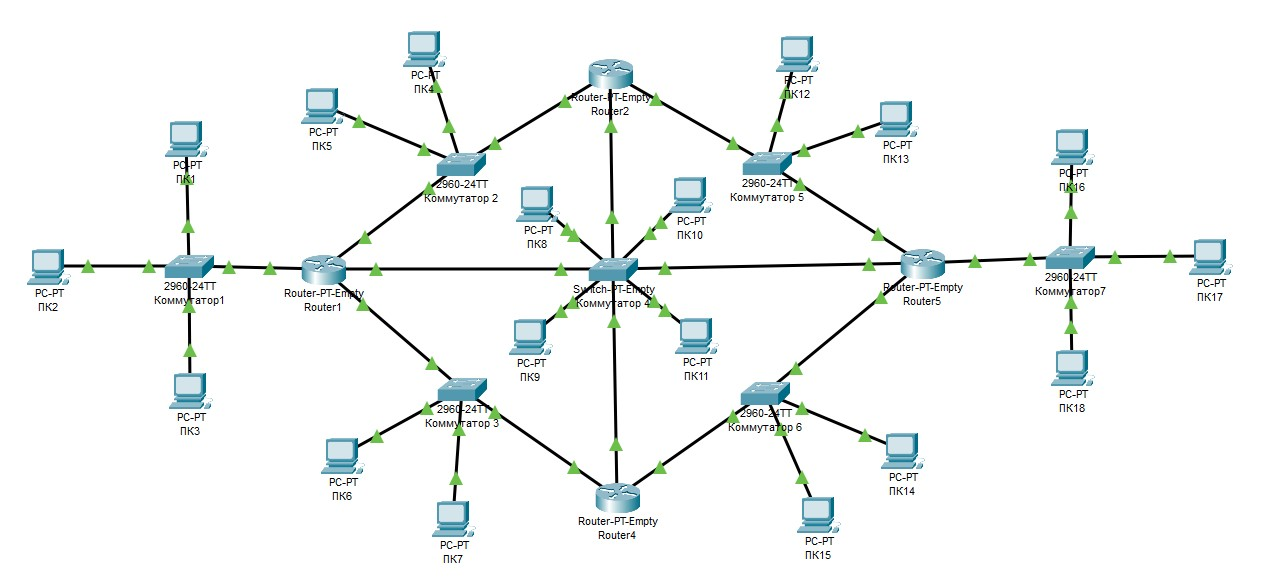
\includegraphics[width=1.\textwidth]{1}
        \caption{Заданная конфигурация}
        \label{fig:image1}
    \end{figure}

    \begin{figure}[H]
        \centering      %размер рисунка       здесь находится название файла рисунка, без указания формата
        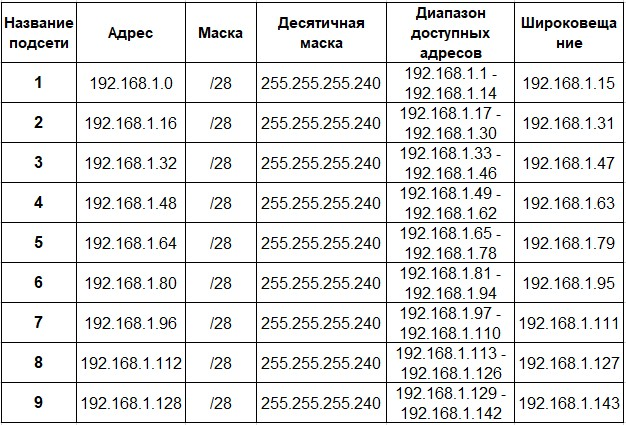
\includegraphics[width=0.8\textwidth]{2}
        \caption{Таблица IP адрессов устройств в заданной конфигурации для случая с одной маской}
        \label{fig:image1}
    \end{figure}

    \begin{figure}[H]
        \centering      %размер рисунка       здесь находится название файла рисунка, без указания формата
        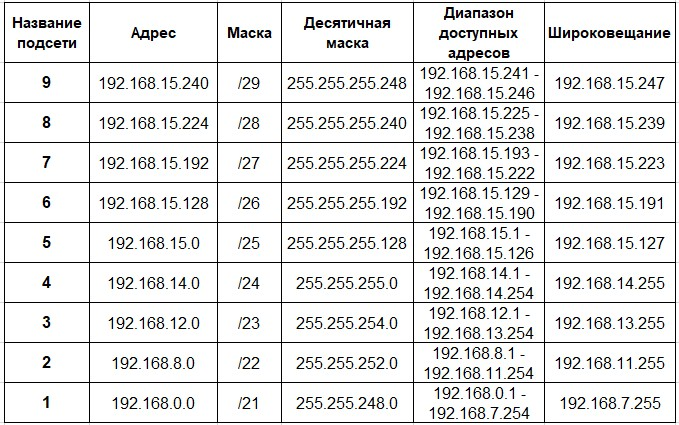
\includegraphics[width=0.9\textwidth]{3}
        \caption{Таблица IP адрессов устройств в заданной конфигурации для случая с разными масками}
        \label{fig:image1}
    \end{figure}

    \item В режиме симуляции Cisco Packet Tracer настроить протокол маршрутизации RIPv1 на каждом роутере. Затем
    
    a) Проследить в пошаговом режиме симуляции и описать изменение протоколом маршрутизации RIP таблиц маршрутизации 
    на каждом роутере.

    \begin{figure}[H]
        \centering      %размер рисунка       здесь находится название файла рисунка, без указания формата
        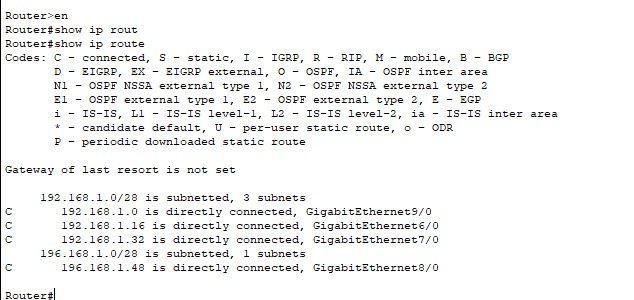
\includegraphics[width=0.9\textwidth]{4}
        \caption{Таблица маршрутизации роутера 1 вначале}
        \label{fig:image1}
    \end{figure}

    Таблица маршрутизации изначально имеет только информацию о подсетях, подключенных напрямую к роутеру, а с течением
    времени протокол RIP, отправляющий каждые 30 секунд пакеты, заполняет таблицу. 

    \begin{figure}[H]
        \centering      %размер рисунка       здесь находится название файла рисунка, без указания формата
        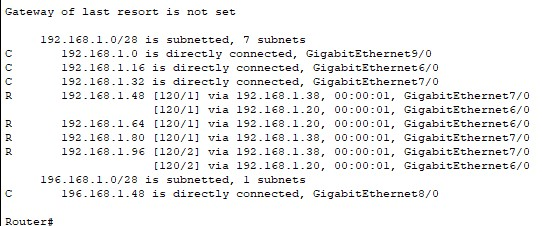
\includegraphics[width=0.9\textwidth]{5}
        \caption{Таблица маршрутизации роутера 1 спустя какое-то время}
        \label{fig:image1}
    \end{figure}

    b) Ответить на вопрос – будет ли одинаково корректно работать протокол маршрутизации RIPv1 для случая с одинаковыми масками 
    и для случая с разными масками? В чем будет проявляться некорректность?
    
    RIPv1 не поддерживает VLSM, поэтому этот протокол будет работать не корректно в случае с разными масками.

    c) Настроить протокол RIPv2 для случая некорректной работы протокола RIPv1 и убедиться в корректности его работы.

    d) Добавить к роутеру Router2 или роутеру Router4 (в режиме симуляции) локальную сеть по аналогии с локальными сетями, в которых 
    расположены ПК2 и ПК17. В режиме симуляции пошагово проследить и описать как протокол маршрутизации RIP будет менять таблицы маршрутизации 
    на каждом роутере в сети и как в итоге распределенная сеть «приспособится» к такому изменению, то есть добавленная сеть будет доступна для 
    сообщений из любой точки, что проверяется с помощью утилиты ping.

    \begin{figure}[H]
        \centering      %размер рисунка       здесь находится название файла рисунка, без указания формата
        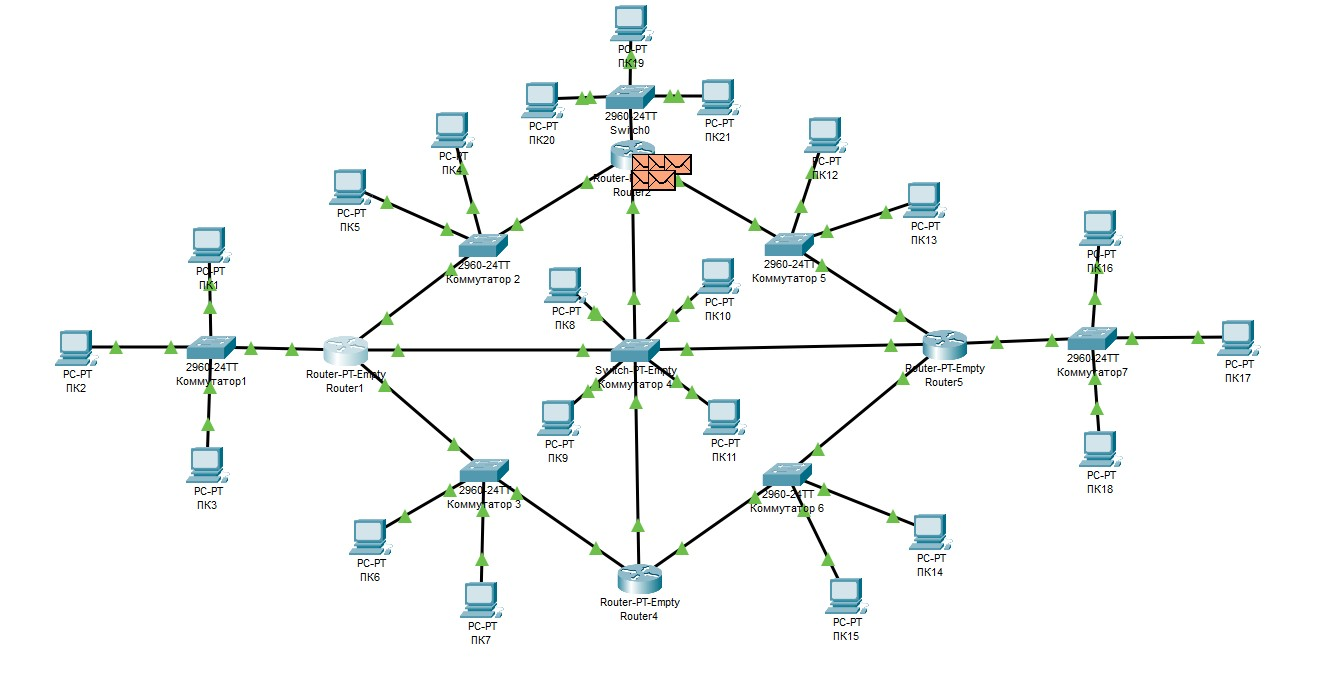
\includegraphics[width=0.9\textwidth]{7}
        \caption{Изменение конфигурации}
        \label{fig:image1}
    \end{figure}

    \begin{figure}[H]
        \centering      %размер рисунка       здесь находится название файла рисунка, без указания формата
        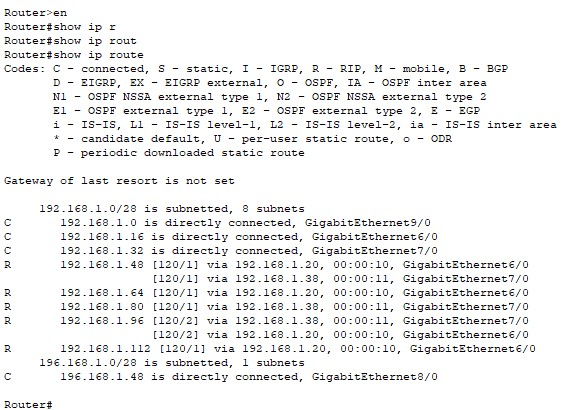
\includegraphics[width=0.7\textwidth]{6}
        \caption{Таблица маршрутизации роутера 1 после подключения новой подсети для случая с одинаковыми масками}
        \label{fig:image1}
    \end{figure}

    \begin{figure}[H]
        \centering      %размер рисунка       здесь находится название файла рисунка, без указания формата
        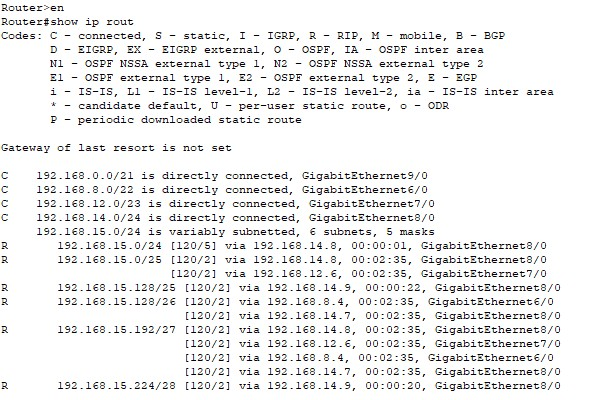
\includegraphics[width=0.7\textwidth]{8}
        \caption{Таблица маршрутизации роутера 1 после подключения новой подсети для случая с разными масками}
        \label{fig:image1}
    \end{figure}

    По аналогии с роутером 1 за счет протокола RIP новая подсеть будет добавлена в таблицу маршрутизации каждого роутера.

    e) Исследовать поведение сети выполнив команду ping с ПК2 до ПК17. Выявить маршруты следования пакетов.

    \begin{figure}[H]
        \centering      %размер рисунка       здесь находится название файла рисунка, без указания формата
        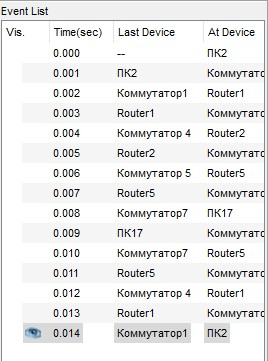
\includegraphics[width=0.4\textwidth]{9}
        \caption{Маршрут следования пакетов для случая с разными масками}
        \label{fig:image1}
    \end{figure}

    \begin{figure}[H]
        \centering      %размер рисунка       здесь находится название файла рисунка, без указания формата
        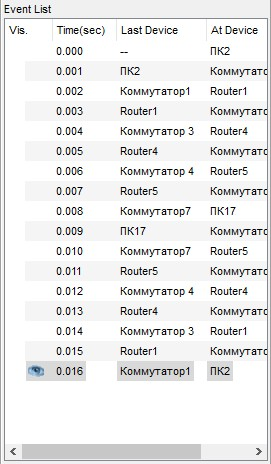
\includegraphics[width=0.35\textwidth]{10}
        \caption{Маршрут следования пакетов для случая с одинаковыми масками}
        \label{fig:image1}
    \end{figure}

    f) Сымитировать техническую неисправность на активном маршруте, отключив один из интерфейсов. Как изменится маршрут и почему?

    \begin{figure}[H]
        \centering      %размер рисунка       здесь находится название файла рисунка, без указания формата
        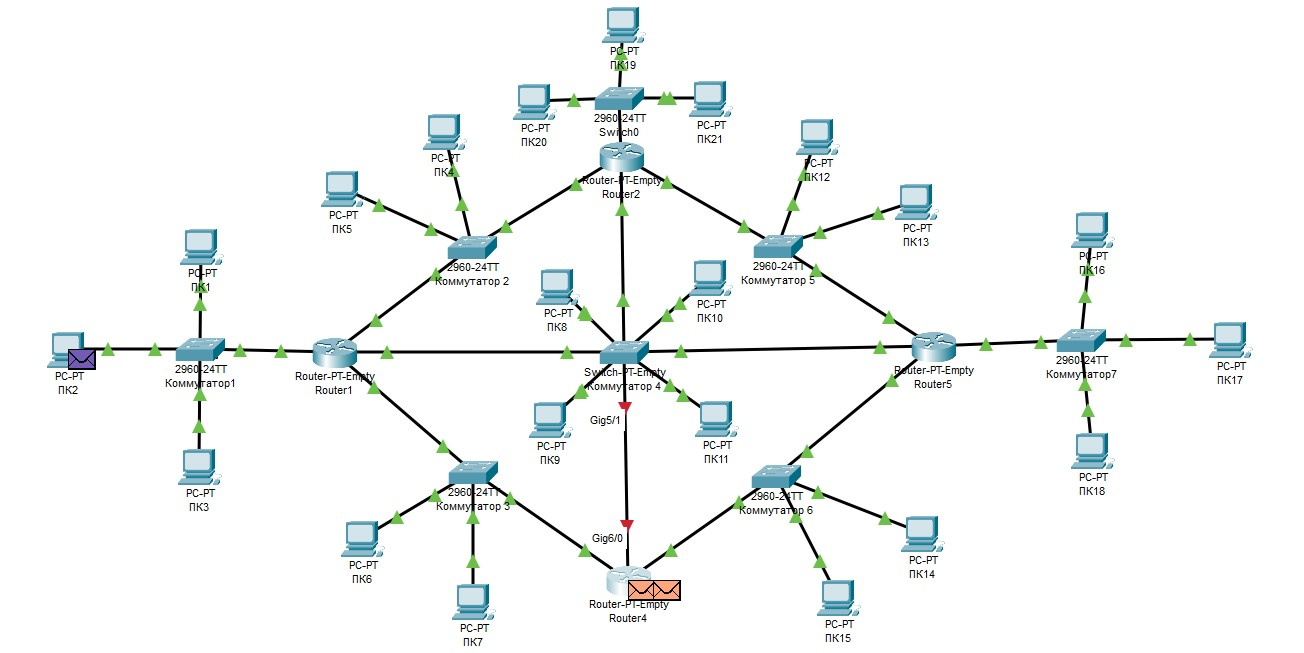
\includegraphics[width=1.\textwidth]{11}
        \caption{Имитация технической неисправности}
        \label{fig:image1}
    \end{figure}

    При имитации технической неисправности пакеты будут следовать по другому маршруту. Как видно на рисунке 11, после отключения одного из 
    интерфейсов на активном маршруте роутер, на котором и произошло отключение, сгенерирует несколько RIP пакетов, которые изменят 
    таблицу маршрутизации других роутеров. Что можно увидеть на примере изменение таблицы первого роутера.

    \begin{figure}[H]
        \centering      %размер рисунка       здесь находится название файла рисунка, без указания формата
        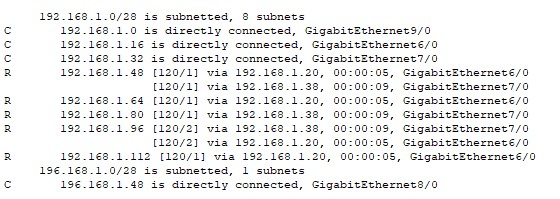
\includegraphics[width=1.\textwidth]{12}
        \caption{Таблица маршрутизации роутера 1 в момент отключения одного из интерфейсов роутера 4}
        \label{fig:image1}
    \end{figure}

    \begin{figure}[H]
        \centering      %размер рисунка       здесь находится название файла рисунка, без указания формата
        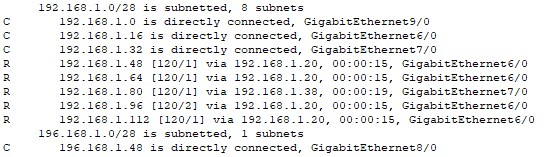
\includegraphics[width=1.\textwidth]{13}
        \caption{Таблица маршрутизации роутера 1 после того, как пакет RIP, отправленный роутером 4, достиг его}
        \label{fig:image1}
    \end{figure}

    За счет этих изменений в таблицах и происходит изменение маршрута следования пакетов.
    
    \begin{figure}[H]
        \centering      %размер рисунка       здесь находится название файла рисунка, без указания формата
        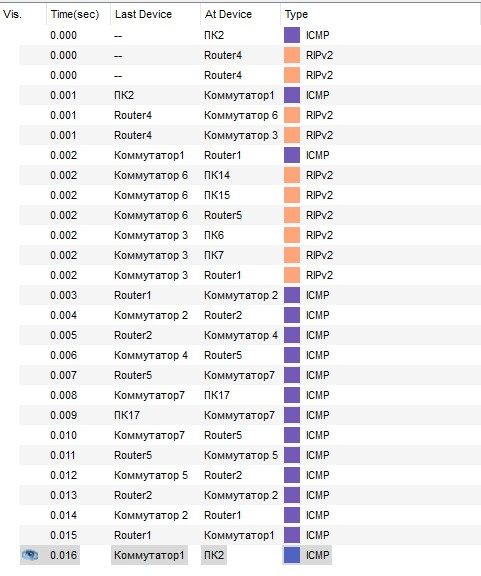
\includegraphics[width=0.6\textwidth]{14}
        \caption{Маршрут следования пакетов после отключения одного из интерфейсов на активном пути}
        \label{fig:image1}
    \end{figure}

    \item Ответить на вопрос – в чем отличие RIPv2 от RIPv1, во всех ли случаях они работают одинаково, какие IP-адреса используются 
    в заголовках RIP-пакетов? Как в случае широковещательной рассылки ПК понимают, что RIP-пакеты адресованы не им?

    RIPv1 не отправляет маску подсети для обновления таблиц маршрутизации, помимо этого он не может отправить пакет на маршрутизаор
    находящийся на растояние 15 узлов, и что самое важное он не поддерживает метод VLSM, все эти минусы были исправлены во 2 версии
    протокола RIP. В заголовке RIPv1 протокола находится адрес 255.255.255.255, в заголовке RIPv2 находится адрес 224.0.0.9. В случае
    широковещательной рассылки в пакете указан порт 520, это значит, что ПК не сможет принять данный пакет. 
    
\end{enumerate}

\end{document}
